\clearemptydoublepage
\chapter{Estado del Arte}
\chaptermark{Estado del Arte}

Organizar información a través de ontologías es muy común en diferentes ámbitos científicos como la biomedicina, informática, filosofía, etc.
Esto ha dado lugar a numerosas opciones de software dedicado a representar dichas ontologías \cite[]{ontologyEditors}. Estos editores se encargan de tareas como creación,
edición, visualización, exploración, \textit{debugging}, etc. Por estas razones, el desarrollo de una aplicación para trabajar con ontologías no es
una tarea sencilla, y requiere de mucho estudio y planeamiento, ya que todas tienen falencias y puntos débiles en distintas etapas del trabajo \cite[]{ontologyIssues}.

Todas las herramientas que podemos encontrar tienen la característica común de trabajar solo en el espacio bidimensional, como la inmensa mayoría de programas hoy en día.
Por esta razón, si queremos expandir el horizonte de la tecnología, debemos empezar a probar qué tan útil es la Realidad Extendida en diferentes ámbitos. En este caso,
vamos a tomar como referencia el software más utiizado con fines de visualización, llamado Protégé.

\begin{figure}[ht]
   \begin{center}
      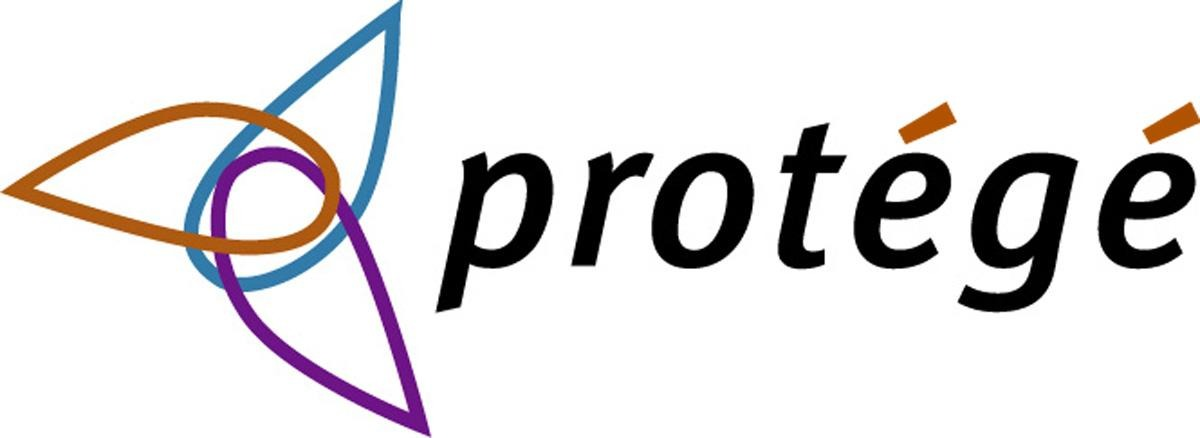
\includegraphics[width=0.7\linewidth]{chapter1/figures/protege.jpg}
   \end{center}
   \caption[Protégé Logo]
   {\footnotesize Protégé Logo}
   \label{fig:mufigure3}
\end{figure}

Es un editor de ontologías gratis y open-source, que provee un esquema de trabajo para construir sistemas inteligentes y se caracteriza
por brindar una útil interfaz de visualización, a diferencia de otros softwares de ontologías. Sin embargo, aprender a operar esta herramienta no es fácil
y requiere bastante tiempo y dedicación \cite[]{ontologyTutorial}.

El principal problema de este tipo de programas, es el rendimienot limitado en grandes ontologías. Aunque Protégé es adecuado para la mayoría de las necesidades de modelado de ontologías, puede experimentar limitaciones de rendimiento al trabajar con ontologías muy grandes o complejas. En tales casos, los usuarios pueden encontrar que el rendimiento de la herramienta se ralentiza o que experimentan problemas de memoria.
Sumado al hecho de que compartir una ontología a través de imágenes o capturas de pantalla en un reporte, complica demasiado la interpretación y no se puede apreciar correctamente lo que se está representando.